\subsection{Materiali}

\begin{sidewaysfigure*}
	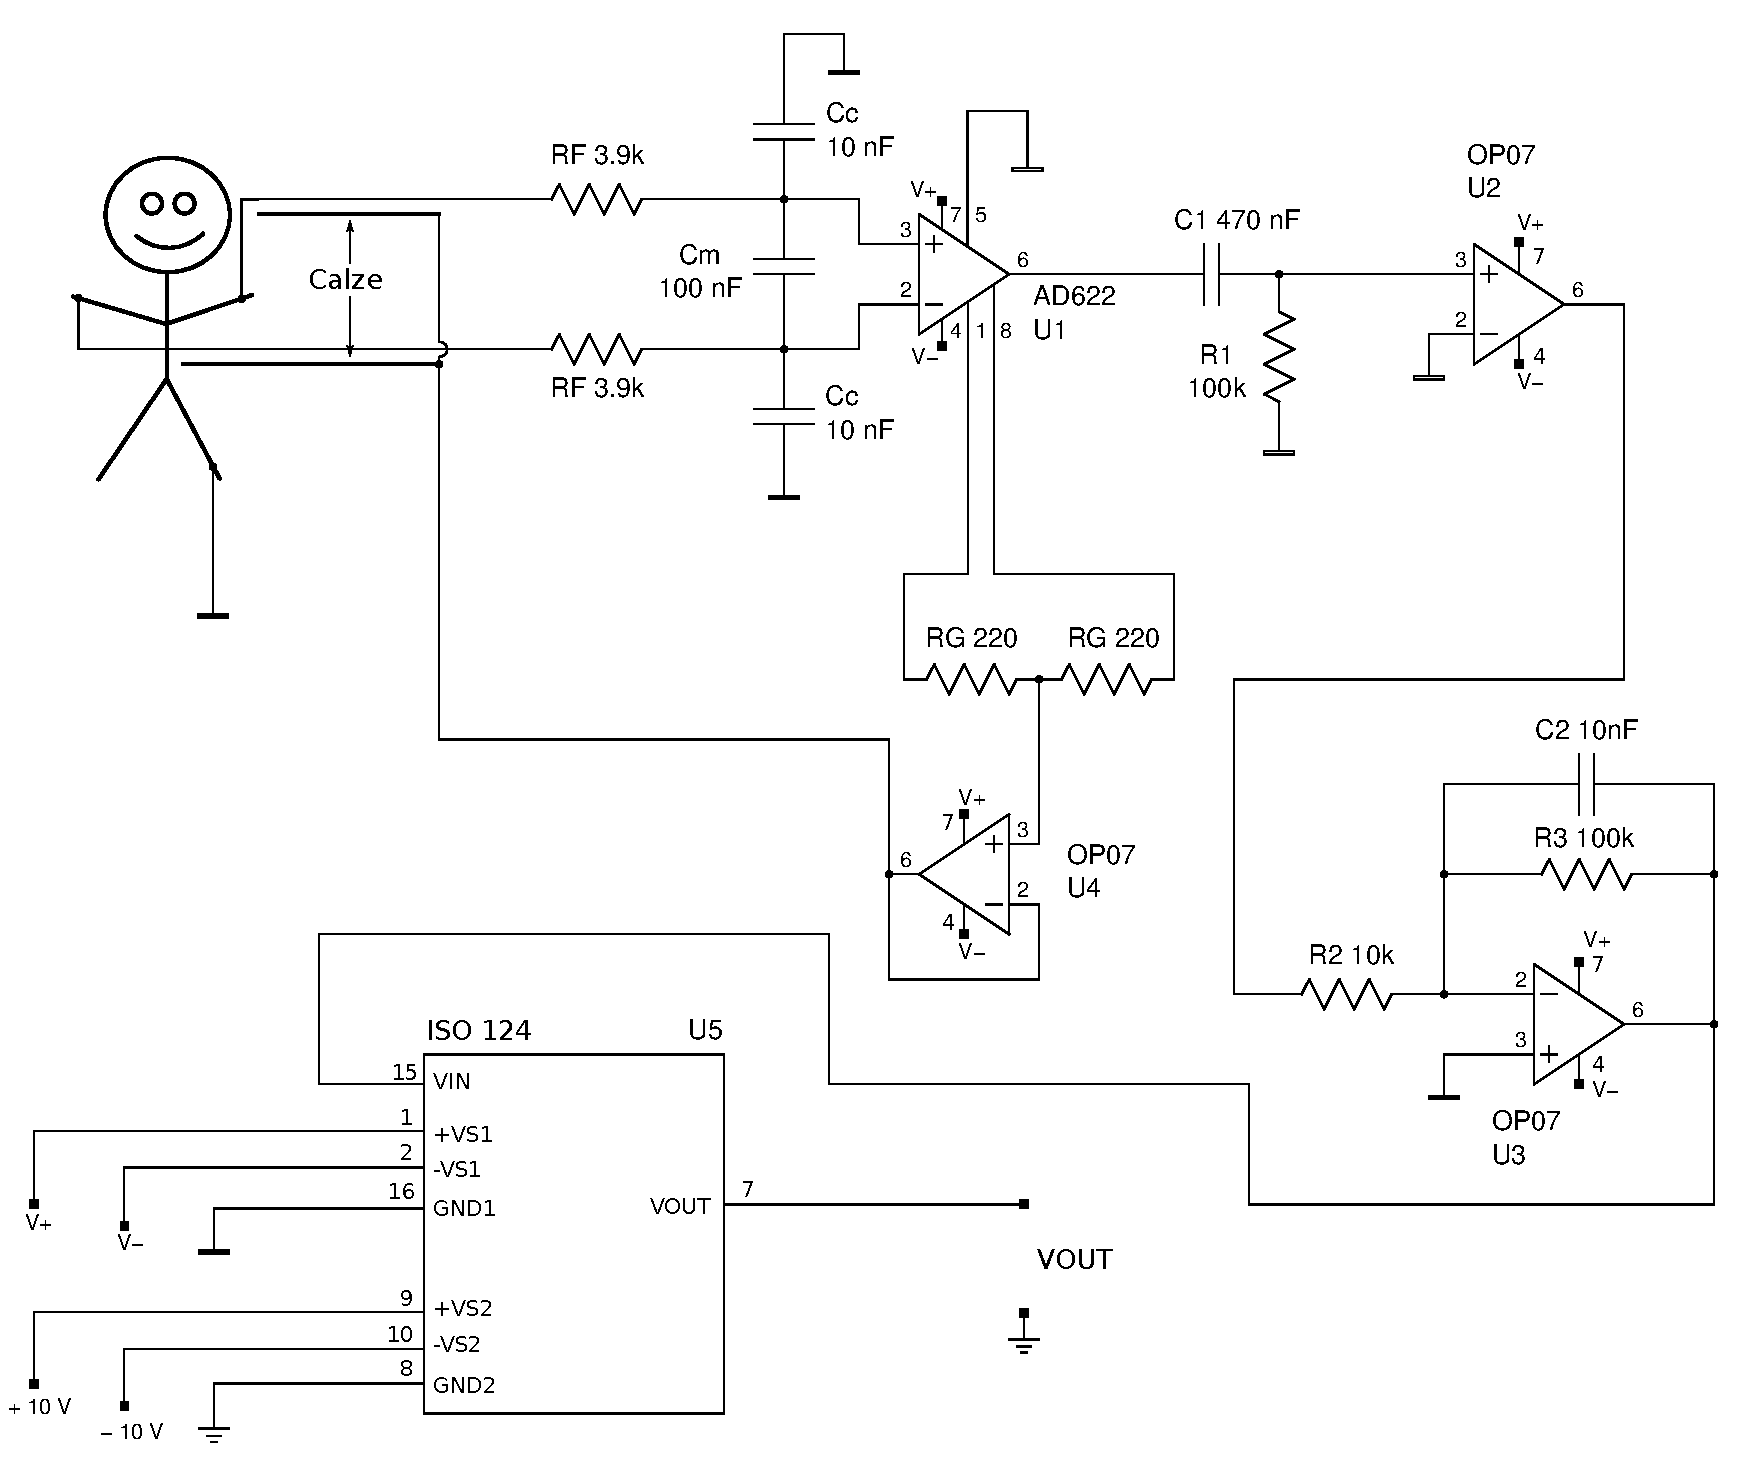
\includegraphics[width=\textwidth]{figure/s.pdf}
    \caption{}
    \label{fig:circ6}
\end{sidewaysfigure*}

\begin{itemize}
    \item{Breadboard, cavi a banana e cavetti da breadboard.}
    \item{3 amplificatori operazionale OP07 e un'amplificatore strumentale AD622.}
    \item{Generatore di tensione di riferimento REF02.}
    \item{Resistenze: \SI{1}{\kilo\ohm}, \SI{1.5}{\kilo\ohm}, \SI{2.2}{\kilo\ohm}, \SI{4.7}{\kilo\ohm}, \SI{10}{\kilo\ohm}, $3 \times$\SI{100}{\ohm}.}
    \item{Potenziometri: $3 \times$\SI{1}{\kilo\ohm}, \SI{10}{\kilo\ohm}}
    \item{Resistenza al platino PT100.}
    \item{Resistenza riscaldante da \SI{27}{\ohm} da 1/2 W.}
    \item{Alimentatore di corrente continua.}
    \item{Generatore di forme d'onda Agilent 33120A.}
    \item{Multimetro Agilent 34410A.}
    \item{Oscilloscopio Agilent DSO-X 2002A.}
\end{itemize}

